\documentclass[letterpaper, 11pt]{article}

\usepackage{amsmath}
\usepackage[final]{graphicx}
\usepackage[left = 1.5in, right =1.5in, top = 1.25in, bottom = 1.25in]{geometry}
\usepackage{booktabs}
\usepackage{tabularx}
\usepackage{longtable}


\title{FTrack v0.9.3\\User's Manual}
\author{Dan Valente\\\small{Mitra Lab}\\\small{Cold Spring Harbor Laboratory}}
\date{\today}

\begin{document}
\maketitle

\section{Introduction}

FTrack is a suite of functions written in Matlab for the purpose of single-object video tracking.
Specifically, the ``single-object" is assumed to be a fruit fly, although this need not be the
case. The current version (v0.9.3) uses the videoIO
toolbox\footnote{\texttt{http://sourceforge.net/projects/videoio/}} to read the videos into Matlab.
At this point FTrack, does not allow for multiple fly tracking and has no analysis functionality.
The analysis functionality is contained within the accompanying program FAnalyze\footnote{See
FAnalyze documentation for details}.  If need be, with small modifications, the FlyTracker function
(which is the backbone for FTrack) will most likely be able to track multiple \emph{well-separated,
non-colliding} flies. FTrack provides the user with the raw tracked data, along with the ability to
view the data, clean any obvious false tracks, and correct for camera tilt. It is up to the user to
smooth and segment the subsequent data anyway that the user sees fit.

The functions were written as generally as possible to locate a
moving object and track the position of that object in each frame.
The algorithm that FTrack employs is relatively basic and was
optimized for the fly tracking application with the video setup used
by our lab. It has only been tested in videos with very simple,
unchanging background conditions (namely a black fly on a white
background or a white fly on a black background).  FTrack is not
guaranteed to work in videos of higher complexity or with different
setups, although it should have a reasonable amount of versatility.

FTrack functions are relatively modular, so the overall structure of
the program can be maintained if changes to any particular function
are required. Those who are Matlab-savvy are encouraged to
modify/replace functions as you see fit. Those who are not
Matlab-savvy should refrain from manipulating the \texttt{.m} files,
and contact the author with any suggestions for additions or
subtractions to the program.  Please note, however, that only the
most relevant, pressing changes will be made.

\section{Overview of the FTrack algorithm}
\label{Overview} The algorithm behind FTrack is relatively rudimentary and is described in detail
in Ref.\ \cite{valente1} and Ref.\ \cite{valente2} The underlying assumption is that the object
moves from frame to frame, and so subtracting a background image will highlight pixels that are
different from this background. FTrack creates a background, subtracts it from the current frame,
and squares each resulting pixel to increase the signal to noise ratio. Then, the brightest pixel
in this image is found and the center of mass (really, center of \emph{intensity}) of a subset of
pixels around this point is calculated.  This center of intensity is used as the object's location.

There are two caveats to this method, and both have to do with the calculation of the background
image. First, in order to find the object in the first frame, a static background image must be
calculated. This background is an average of the first $N_B$ frames, where $N_B$ is a user-defined
parameter. $N_B$ should be relatively small so that the algorithm does not take an exorbitant
amount of time to read the video and calculate the average, but needs to be large enough to ensure
at least some variation in the image.\footnote{We have seen that 100-500 frames gives reasonable
results, depending on frame rate and activity of the fly.}

After the first two frames, the background is calculated by taking a weighted running average
$$I_{B}(n+1) = \alpha I_{B}(n) + (1-\alpha)I(n)$$
where $I_B$ is the background image, $I$ is the current frame, $\alpha$ is the weighting parameter
(between 0.90 and 1.00), and $n$ is the frame index.  The entire image is updated \emph{except} for
a square region that includes the fly.  This allows the algorithm to work effectively even when the
fly remains stationary for a long period of time.

The body axis of the object is also calculated as the tracking algorithm proceeds.  To do this,
pixels in the difference image with intensities greater than 20\% of the maximum intensity define a
2D projection of the object.  This projection is effectively a scatter plot, with points placed at
the locations of the pixels that define the object. A Principle Components Analysis (PCA) is then
performed on this data. Since a fly is typically longer than it is wide, the component with the
largest variance is used to calculate the orientation angle $\phi_1$. The orientation angle is
somewhat ambiguous, since $\phi_2 = \phi_1+\pi$ defines the same axis. For ease of use, the program
divides up the orientation angles into two groups, $\phi_{UHP}$ and $\phi_{LHP}$.  $\phi_{UHP}$ is
defined as the orientation angles that lie in the upper half plane ($0 < \phi < \pi$) and
$\phi_{LHP}$ are angles that lie in the lower half plane($-\pi < \phi < 0$). For each frame, both
angles are available to the user.  By comparison of these angles with the direction of velocity,
one can reasonably estimate in which direction the object is moving. It is up to the user to decide
which orientation angle to choose.

\section{Placing FTrack in the Matlab path}
In order to use FTrack, the FTrack folder must first be placed in the Matlab path.  It is also
recommended to remove any previous versions of FTrack from the Matlab path.

\begin{enumerate}
\item Open Matlab.
\item Select \textbf{File $>>$ Set Path\ldots} from the toolbar.  The Set Path dialogue will open up.
\item Click on the \textbf{Add Folder\ldots} button.
\item Find the FTrack directory and select the \textbf{functions} folder. Click \textbf{OK}.  The path and name of the FTrack
functions folder should show up in the Matlab search path window.
\item Find the videoIO folder that fits your Matlab release.  FTrack has only been tested for R2006a, R2006b, and R2007a.  For other releases, you will need to recompile the videoIO functions (see the videoIO documentation if you need to do this).
\item Repeat Step 4 with the appropriate \textbf{videoIO} folder.
\item Click \textbf{Save}, and then click \textbf{Close}. FTrack is now ready to use.  To test if
it is installed correctly, type \texttt{help videoReader} and then \texttt{help FTrack} in the
Matlab command window. If an error is obtained upon either of these commands, the folders were not
correctly installed, so try to re-install.  If the installation worked, you will be able to open
the program or use any of the functions regardless of what directory you are currently in.
\end{enumerate}


\section{The FTrack GUI}
The FTrack graphical user interface (GUI) was written to facilitate use of the tracking functions.
It is specifically intended for users who have minimal-to-no experience with programming in Matlab.
Because it provides an accessible interface for loading and tracking, use of the GUI is recommended
for all applications unless the user prefers to incorporate specific functions into his/her own
scripts.

The interface is shown in Fig.\ \ref{GUI} and is divided into two general sections: Tracking and
View \& Clean Data.  The functionality of these sections is described below.

\begin{figure}
    \centering
    \hspace{-0cm}
    \includegraphics[bb= 0.0 0.0 613.0 341.0 clip=true, scale = 0.7]{GUI.jpg}
    \caption{The FTrack GUI}
    \label{GUI}
\end{figure}


\subsection*{Instructions for Tracking}
The first section of the GUI is the ``meat" of the program, so to speak.  In this section, the user
inputs all of the necessary information and parameters required to initiate the tracking.

\begin{enumerate}
\item Open Matlab.

\item Type \texttt{FTrack} to start the program.  The FTrack GUI should appear.

\item Click the \textbf{Press to Load Videos} button.  The user can select one or more videos to track (.avi, .mpg, mp2,
etc.).  The name of the videos will appear in Matlab Command window.  If multiple videos are
selected, they will be tracked in succession, and necessary information from each video will be
saved as a .mat file (see below).

\item Click the \textbf{Single Frame Viewer} button.  This will show the first frame of each
selected video; the filename of the particular video can be seen in the title bar of each figure
window. The purpose of having this button is to extract pertinent information about the specific
videos in question and to make sure that they can be read properly by the program.  Information
about the video will be displayed in the Command Window (video dimensions, number of frames, and
frame rate).

\item Click the \textbf{Arena Dimensions} button. When this button is clicked, the user is able to select any number of points in the image by left
clicking.  The user is expected to click points that define the boundary of the arena.  FTrack
assumes a circular/elliptical arena, so it goes ahead and calculates the best fit
ellipse\footnote{The function \texttt{fit\_ellipse} is used for this calculation.  It can
originally be found at
\texttt{http://www.mathworks.com/matlabcentral/fileexchange/loadFile.do?objectId=3215\&objectType=File}}
to the selected points when the user hits Enter.  FTrack then calculates a mask so that only the
portion of the video within the elliptical boundary is tracked.  The resulting mask is shown, along
with the location of the boundary.  Furthermore, the parameters of the resulting ellipse are
displayed in the Command Window. This step \emph{must} be performed if the user plans to employ the
Tilt Correction functionality of FTrack.

\item Select the characteristics of the object in your video: black dot on a white background or a
white dot on a black background. As of this version, each video must have the same characteristics.

\item Click the \textbf{Input Parameters} button.  A window will open with several input boxes.  The filename of the video that
these input parameters correspond to is displayed at the top of this window.
\begin{itemize}
\item Enter the name of the directory where you would like the output files to be stored.
\item Enter the \textbf{Start Frame} and \textbf{End Frame} of the region of video that you would
like to track. Please note that the first frame of a video is indexed as frame 0.
\item Enter the \textbf{Initial background size}.  The need for this number was
discussed in Section \ref{Overview}.  The default is 100 frames, and this should be sufficient for
most applications.
\item Enter the \textbf{Radius of the Arena (in cm)} as well as the \textbf{Bounding box half-size (in
pixels)}.  The Bounding box half-size defines the size of a box
around the fly that will not be updated in the background
calculations (described above).  Make sure this number is slightly
larger than the maximum length of your fly.
\item Enter a value for the \textbf{Background weight} $\alpha$ between 0.9 and 1.0.  The
default (0.9) should be sufficient.
\item Click \textbf{OK}
\item Repeat these steps for each video that you have selected.  Note: it may be helpful to keep
the figure windows from the single frame viewer open while you input parameters.
\end{itemize}



\item Click the \textbf{Track Videos} button to begin tracking.  The progress of the algorithm will
be displayed in the Command Window. After each video is tracked, the raw (x,y) trajectory, time
vector, video information (frame rate, size, etc.), and input data are saved in a \texttt{.mat}
file with the same filename as the video.  The variables saved are described in the Appendix. The
x,y data are also saved as \texttt{.xy} file as a simple two column list of positions, and the
upper half plane orientation data are saved as a .ori file. This allows the user to track many
videos at once and access the data at a later time for processing. The saving happens
\emph{automatically} at the end of tracking, so the user need not worry about it.  A message will
be displayed in the Command Window validating the saving process and completion of the tracking.


\subsection*{View \& Clean Data}
At this point, the user can choose to view and/or clean any trajectory data that has been saved in
a \texttt{.mat} file from a previous tracking session.  You may only select one file to view/clean
at a time. To load in a previously saved session, click the \textbf{View Trajectories} button, and
select a file. A figure will be displayed for the chosen video.  This figure shows the x-position
as function of time (upper left), the y-position of the fly as a function of time (lower left) and
the resulting trajectory (right) as if it were drawn on a video frame.  See Figs.\
\ref{ViewTrajFig} and \ref{exframe} for details.


\subsubsection*{Cleaning the Trajectory} In some cases, the object may leave the frame or hide
behind an obstacle in the environment\footnote{Assuming, of course, measures were not taken to
minimize these events in the experimental setup.}. When this happens, the algorithm is no longer
able to locate the object and will result in a false track for that frame. These false tracks are
marked by regions of the $x$ or $y$ trajectories that are visibly deviant from the ``actual"
trajectory. Definitions of such deviations are largely chosen at the discretion of the user, and
examination of the data will suggest whether these points are actual outliers or are actual
movements of the object. In any case, FTrack allows one to ``clean" these outliers from the data
and interpolate between known true points.  The $x$ and $y$ data must be cleaned separately.
\end{enumerate}

\begin{figure}[p]
 \centering
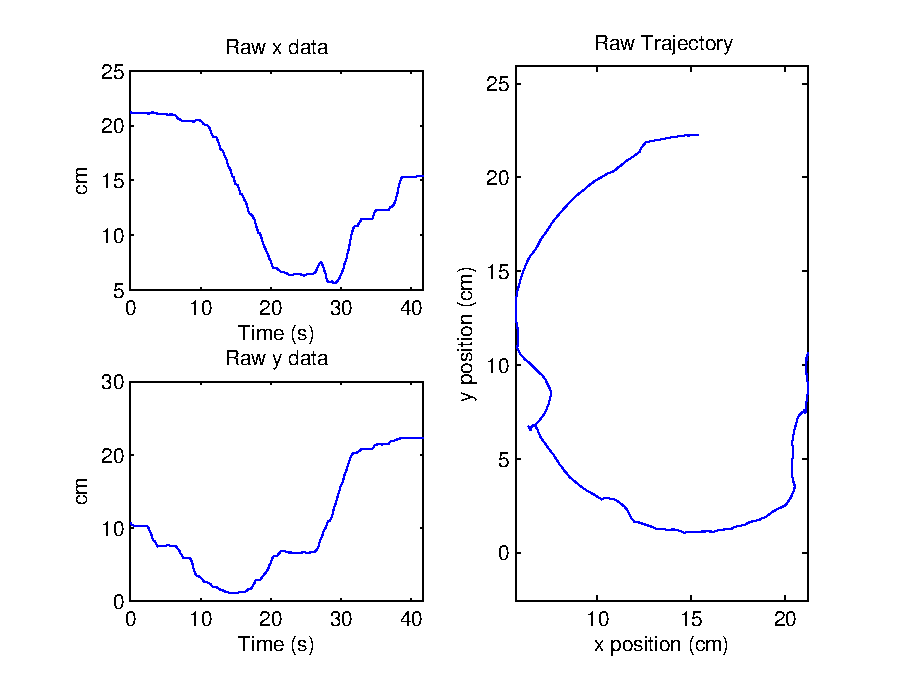
\includegraphics[clip=true, height=3.5in]{ExViewTraj.eps}
\caption{An example figure that will be displayed when the
\textbf{View Trajectory} button is clicked.  The raw $x$ data is
shown in the upper left, the raw $y$ data is shown in the lower
left, and the raw trajectory is shown on the right.}
\label{ViewTrajFig}
\end{figure}
\begin{figure}[p]
 \centering
\includegraphics[clip=true, height=3in]{exframe.eps}
\caption{Dimensions associated with a video frame.  The origin is
defined as (0 cm, 0 cm).  An example trajectory is shown.}
\label{exframe}
\end{figure}

\begin{figure}[p]
 \centering
\includegraphics[clip=true, height = 3.5in]{ExDirtyRegion.eps}
\caption{An example figure showing a section of bad tracks.  The
true trajectory can be inferred from surrounding data.  Also shown
on the figure are the definitions for the region of data to clean,
the baseline, and the threshold to be chosen.}
 \label{ExDirtyRegion}
\end{figure}
\begin{figure}[p]
 \centering
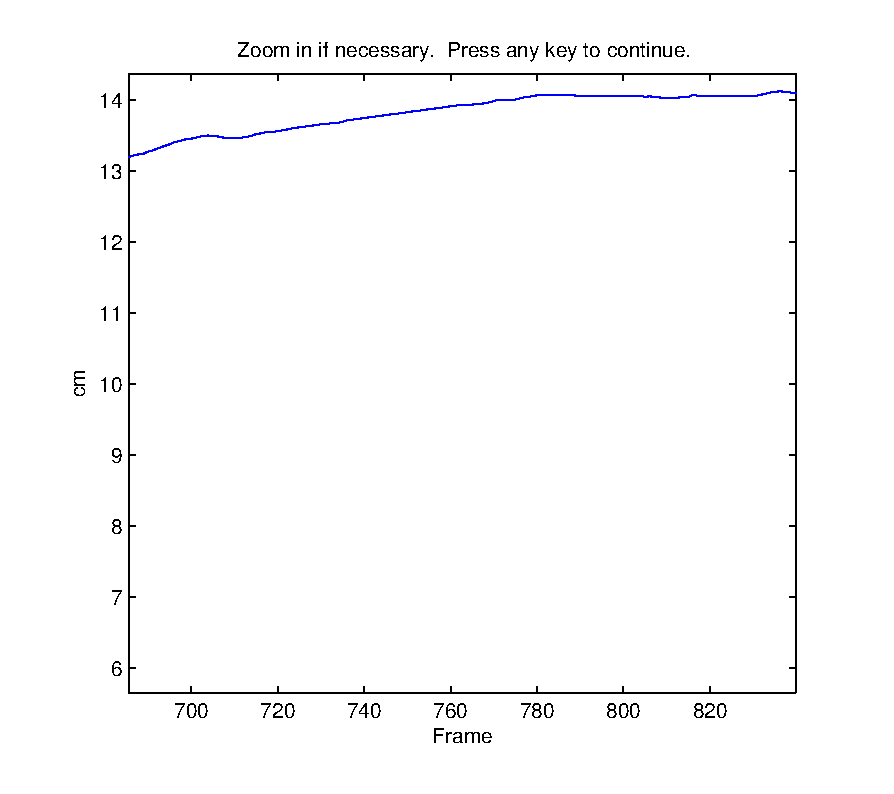
\includegraphics[clip=true, height = 3.5in]{ExCleanRegion.eps}
\caption{The result of cleaning the region in Fig.
\ref{ExDirtyRegion}.} \label{ExCleanRegion}
\end{figure}

\begin{enumerate}
\item Click \textbf{Clean x data} or \textbf{Clean y data}.  A window will appear with the
requested data.
\item Use the zoom tools in the toolbar of the figure window examine any areas of interest in
further detail.  This will help you determine whether points are false tracks or true movements and
will ensure that you only clean the regions where false tracks exist.
\item Press any key to continue.
\item Crosshairs will appear in the figure window.  These will allow you to select the region of data you wish to clean.
\item Select a point to the left of the false data, then select a point to the right of the false
data. This defines the region to clean.
\item Select a point near the apparent actual trajectory.  This is called the baseline.  Then
select a point that defines a threshold for the outliers; that is, a point above or below which any
existing data will be discarded.  If the threshold is below the baseline, the function will discard
data below the threshold; if the threshold is above the baseline, points above the threshold will
be discarded. See the example in Figs. \ref{ExDirtyRegion} and \ref{ExCleanRegion}.
\item  The cleaned data will immediately appear.  At this point, you can zoom out to clean another
section of data, or press Return twice to escape.   The figure will automatically close. A message
will be displayed in the Message Center letting you know that the data has been cleaned.  \emph{DO
NOT close the figure window without pressing Return twice!}
\end{enumerate}


\subsubsection*{Tilt Correction}

\textbf{Note: As of this version (0.9.3), tilt correction is implemented in a slightly different
way than discussed in Ref. \cite{valente1}.  The current method should be more robust.}

When this button is pressed, FTrack takes the ellipse data from the Arena Dimensions calculation
and transforms the data so that the arena becomes approximately circular. First the ellipse is
centered at (0,0).  Then, the ellipse is rotated such that the elliptical axis closest to the
x-axis rotates onto the x-axis.  Finally, the semiminor axis of the ellipse is stretched to the
length of the semimajor axis, creating a circle.

After the transformation, the data lies within a circle centered approximately at the point (0,0).
The data is then converted from pixels into centimeters using the radius that the user has
previously input.  A figure appears that shows the transformed trajectory with the transformed
arena boundary. Finally, the transformed data is saved.

CAUTION: It is recommended to backup the trajectory .mat file before
hitting the Tilt Correction button.  There currently is no
functionality for preventing overwriting of good x,y pixel data if
something has gone awry in the transformation process (such as if
the user selected bad boundary after hitting the Arena Dimensions
button).

\section{Known Problems}
The only problem encountered so far in v0.9.3 is that the reading of a frame sometimes fails
towards the end of very long videos.  This means that the numFrames field in the VideoInfo
structure does not actually correspond to the number of frames that you can successfully track with
FTrack, and FTrack will crash before finishing and saving. The current solution to this is as
follows: Download the video-editing program VirtualDub (http://www.virtualdub.org/). Load the video
into VirtualDub and notice what the last frame is (move the time slider all the way to the right).
This corresponds to the last frame that FTrack will be able to read as well.  We are currently
working on making FTrack able to catch the error before it crashes.

\section{Concluding Comments}
For those who wish to use the functions from the Matlab command line, complete descriptions of
their use and workings can be found in the Matlab help files; simply type \texttt{help
function\_name}. Describing them in detail here would be superfluous.  The scripts are also highly
commented, and as such, they should be relatively easy to follow. Suggestions for improvements to
the algorithms, the GUI or the coding style are highly encouraged!  Comments on the ease of use of
the GUI and functions are also important for refining this program.  Since this is v0.9.3, FTrack
needs a little more testing in order to find all of the bugs (pun intended).  Once sufficient
testing has been performed, we hope to release an honest to goodness v1.0.  Until then, please
check and double-check any results that you obtain from this program, and make sure that they make
sense! \\

\noindent Enjoy!


\section{Appendix: Variables saved in the \texttt{.mat} file}

The following is a list of the variables saved to the .mat file with the same filename as the
tracked video (minus the extension!).

\begin{center}
\begin{longtable}{ p{5cm}  p{8cm} }
    \texttt{t} & Time vector in seconds\\
    \texttt{x} & x-position of the fly in centimeters\\
    \texttt{y} & y-position of the fly in centimeters\\
    \texttt{orientation}& 2 x N vector, where N is the number of frames.  The first row contains the UHP orientation data; the second row contains
    the LHP orientation data.\\


    \texttt{arena} & structure that defines the best fit elliptical boundary of the arena (see \texttt{fit\_ellipse} help file.  The arena structure has the
    following fields: \begin{itemize} \item \texttt{a}: sub axis (radius in pixels) of the X axis of the non-tilt ellipse
    \item \texttt{b}:   sub axis (radius in pixels) of the Y axis of the non-tilt ellipse
    \item \texttt{phi}: orientation in radians of the ellipse (tilt)
    \item \texttt{X0}: center at the X axis of the non-tilt ellipse (in pixels)
    \item \texttt{Y0}: center at the Y axis of the non-tilt ellipse (in pixels)
    \item \texttt{X0\_in}: center at the X axis of the tilted ellipse (in pixels)
    \item \texttt{Y0\_in}: center at the Y axis of the tilted ellipse (in pixels)
    \item \texttt{long\_axis}: size of the long axis of the ellipse (in pixels)
    \item \texttt{short\_axis}:size of the short axis of the ellipse (in pixels)
    \item \texttt{status}: status of detection of an ellipse
    \item \texttt{epsilon}: the eccentricity of the ellipse
    \item \texttt{psi}: angle of tilt of the camera (radians)
    \item \texttt{semiminor}: the semiminor axis of the ellipse (in pixels)
    \item \texttt{semimajor}: the semimajor axis of the ellipse (in pixels)
    \item \texttt{boundaries}: N x 2 vector of points describing the boundary (x,y) (in pixels)
    \end{itemize}\\
    \texttt{VideoInfo} & The VideoInfo structure
    has the following fields: \begin{itemize} \item \texttt{url}: the filename of the video \item
    \texttt{fps}: the frame rate of the video \item \texttt{width}: the width of the video (in
    pixels) \item \texttt{height}: the height of the video (in pixels) \item \texttt{bpp}:  See
    videoIO documentation  \item \texttt{type}: See videoIO documentation \item \texttt{numFrames}:
    number of frames in the video \item \texttt{fourcc}: See videoIO documentation \item
    \texttt{nHiddenFinalFrames}: See videoIO documentation\end{itemize}\\
    \texttt{InputData} & The InputData structure
    has the following fields: \begin{itemize} \item \texttt{OutputPath}:  the name of the directory
    where output files are to be stored (.mat, .xy, and .ori files). \item \texttt{StartFrame}:
    the frame where tracking begins. \item \texttt{EndFrame}: the frame where tracking ends. \item
    \texttt{NBackFrames}: the number of frames in the initial background calculation \item \texttt{pixels\_in\_cm}: the number of pixels in 1 centimeter (only saved if tilt correction
performed)
    \item \texttt{sqrsize}: the
    bounding-box half width (described above) \item \texttt{alpha}: the background weighting
    parameter (described above)\end{itemize}\\



\end{longtable}
\end{center}



\begin{thebibliography}{9}
\bibitem{valente1}Valente, D., Golani, I., and P.P. Mitra, ``Analysis of the trajectory of \emph{Drosophila
melanogaster} in a circular open field arena." PLoS ONE 2(10), e1083
doi:10.1371/journal.pone.0001083, (2007)
\bibitem{valente2}Valente, D., Wang H., Andrews P., Saar S., Tchernichovski O., Benjanimi, Y., Golani I. and
P.P. Mitra, ``Characterization of animal behavior through the use of audio and video signal
processing." IEEE Multimedia, 14 (2), 32-41, (2007)
\end{thebibliography}

\end{document}
